\documentclass[twoside]{ctuthesis}

\ctusetup{
	%preprint = \ctuverlog,
	mainlanguage = english,
	title-english = {Machine learning for saturation-based theorem proving},
	doctype = D,
	faculty = F3,
	department-english = {\href{https://cyber.felk.cvut.cz/}{Department of Cybernetics}},
	author = {Mgr. Filip Bártek},
	supervisor = {\href{https://people.ciirc.cvut.cz/~urbanjo3/}{Mgr. Josef Urban, Ph.D.}},
	% TODO: Set the correct supervisor address.
	supervisor-address = {Czech Technical University in Prague\\Czech Institute of Informatics, Robotics and Cybernetics.\\Jugoslávských partyzánů 1580/3\\160 00 Praha 6\\Czech Republic},
	supervisor-specialist = {\href{https://people.ciirc.cvut.cz/~sudamar2/}{RNDr. Martin Suda, Ph.D.}},
	% https://intranet.fel.cvut.cz/cz/vv/doktorandi/obory.html
	fieldofstudy-english = {Computer Science},
	keywords-english = {\acrlong{ml}, \acrlong{atping}},
	keywords-czech = {strojové učení, automatické dokazování},
	% TODO: Set the correct date.
	day = 30,
	month = 6,
	year = 2024,
	specification-file = {NavrRamcovehoTematuDP_MS.pdf},
	front-list-of-figures = false,
	front-list-of-tables = false,
	pkg-hyperref = true,
}

% glossaries must be loaded after hyperref
\usepackage[toc]{glossaries}
\makeglossaries
\glsenablehyper

% The glossary chapter is automatically added into ToC even without the "toc" option.
\glstocfalse

% Logic
\newglossaryentry{PropositionalLogic}{name={propositional logic}, description={?}}
\newglossaryentry{fo}{name={first-order}, description={TBA}}
\newacronym{fol}{FOL}{first-order logic}
\newacronym{hol}{HOL}{higher-order logic}
% TPTP division: "clause normal form"
\newacronym{cnf}{CNF}{clause normal form}
\newacronym{nnf}{NNF}{negation normal form}

% Automated reasoning
\newglossaryentry{ar}{name={automated reasoning}, description={TBA}}
\newacronym{atper}{ATP}{automatic theorem prover}
\newglossaryentry{tper}{name={theorem prover}, description={TBA}}
\newglossaryentry{tping}{name={theorem proving}, description={TBA}}
%\newacronym{atping}{ATP}{automatic theorem proving}
\newglossaryentry{atping}{parent=tping, name={automatic \gls{tping}}, description={TBA}}
\newglossaryentry{saturation}{name={saturation}, description={TBA}}
\newglossaryentry{AxiomSelection}{name={axiom selection}, description={TBA}}
\newacronym{kb}{KB}{Knuth-Bendix}
\newacronym{kbo}{KBO}{Knuth-Bendix \glslink{to}{ordering}}
% Vampire option: --term_ordering (-to)
\newglossaryentry{to}{name={simplification ordering on terms}, description={\gls{term} ordering used to orient equations in \glslink{SuperpositionCalculus}{superposition} inferences and inform \gls{LiteralSelection}}}
\newglossaryentry{superposition}{name={superposition}, see=SuperpositionCalculus, description={?}}
\newglossaryentry{SuperpositionCalculus}{name={superposition calculus}, description={TBA}}
\newglossaryentry{precedence}{name={precedence}, description={?}}
% Vampire option: --symbol_precedence (-sp)
\newglossaryentry{sp}{name={symbol precedence}, parent=precedence, description={permutation of the \gls{signature}}}
\newglossaryentry{signature}{name={signature}, symbol={$\Sigma$}, description={set of all symbols used in a \gls{problem}}}
\newglossaryentry{problem}{name={problem}, description={a set of premises and a conjecture, all of which are specified as formulas}}
\newglossaryentry{LiteralSelection}{name={literal selection}, description={TBA}}
\newglossaryentry{ClauseSelection}{name={clause selection}, description={TBA}}
\newglossaryentry{clause}{name={clause}, description={multiset of \glspl{literal}}}
\newglossaryentry{literal}{name={literal}, description={an \gls{atom} or the negation of an \gls{atom}}}
\newglossaryentry{atom}{name={atom}, description={an application of a \gls{predicate}}}
\newglossaryentry{term}{name={term}, description={TBA}}
\newglossaryentry{symbol}{name={symbol}, description={?}}
\newglossaryentry{predicate}{parent=symbol, name={predicate}, description={a symbol that represents a functional propositional variable}}
\newglossaryentry{function}{parent=symbol, name={function}, description={a symbol that represents a functional variable}}
\newglossaryentry{variable}{name={variable}, description={TBA}}
\newglossaryentry{strategy}{name={strategy}, description={a configuration of an \gls{atper}}}
\newglossaryentry{StrategySchedule}{name={strategy schedule}, description={TBA}}
\newglossaryentry{vampire}{name={Vampire}, description={a prominent \gls{atper}}}
\newglossaryentry{enigma}{name={ENIGMA}, description={?}}

\newglossaryentry{recommender}{name={recommender}, description={TBA}}
\newglossaryentry{PrecedenceRecommender}{name={precedence recommender}, parent=recommender, description={TBA}}
\newglossaryentry{npr}{name={neural precedence recommender}, parent=PrecedenceRecommender, description={TBA}}
\newacronym{ltr}{LTR}{learning to rank}
\newacronym{np}{NP}{nondeterministic polynomial}

% Machine learning
\newacronym{nn}{NN}{neural network}
\newacronym[parent=nn]{ann}{ANN}{aritificial \acrlong{nn}}
\newacronym[parent=nn]{cnn}{CNN}{convolutional \acrlong{nn}}
\newacronym{dl}{DL}{deep learning}
\newacronym[parent=nn]{dnn}{DNN}{deep \acrlong{nn}}
\newacronym[parent=nn]{gnn}{GNN}{graph \acrlong{nn}}
\newacronym[parent=nn]{rnn}{RNN}{recursive \acrlong{nn}}
\newacronym{ml}{ML}{machine learning}
\newglossaryentry{LinearRegression}{name={linear regression}, description={?}}

% Conferences
\newacronym{cade}{CADE}{Conference on Automated Deduction}
\newacronym{ijcar}{IJCAR}{International Joint Conference on Automated Reasoning}
\newacronym{lpar}{LPAR}{International Conference on Logic for Programming, Artificial Intelligence and Reasoning}
\newacronym{paar}{PAAR}{Workshop on Practical Aspects of Automated Reasoning}

\newacronym{aac}{AAC}{automated algorithm configuration}
\newacronym{as}{AS}{algorithm selection}
\newglossaryentry{AlgorithmScheduling}{name={algorithm scheduling}, description={?}}
\newacronym{erc}{ERC}{European Research Council}

\newacronym{asp}{ASP}{answer set programming}
\newacronym{cpu}{CPU}{central processing unit}
\newacronym{mi}{Mi}{megainstruction}
\newacronym{par}{PAR}{penalized average runtime}
\newacronym{pcs}{PCS}{parameter configuration space}
\newacronym{sat}{SAT}{propositional satisfiability}
\newacronym{smt}{SMT}{satisfiability modulo theories}
\newacronym{tptp}{TPTP}{Thousands of Problems for Theorem Provers}
\newacronym{ucb}{UCB}{upper confidence bound}

% Czech Technical University
%\newacronym{ciirc}{CIIRC}{\href{https://www.ciirc.cvut.cz/}{Czech Institute of Informatics, Robotics and Cybernetics}}
%\newacronym{ctu}{CTU}{\href{https://www.cvut.cz/}{Czech Technical University in Prague}}
%\newacronym{fel}{FEL}{\href{https://fel.cvut.cz/}{Faculty of Electrical Engineering}}

% CASC
\newacronym{casc}{CASC}{CADE \acrshort{atper} System Competition}
\newacronym[parent=casc]{casc-14}{CASC-14}{\Acrshort{cade}-14 \acrshort{atper} System Competition}
\newacronym[parent=casc]{casc-j11}{CASC-J11}{11th \acrshort{ijcar} \acrshort{atper} System Competition \cite{DBLP:journals/aicom/SutcliffeD23}}
% https://www.tptp.org/CASC/J11/Design.html#Divisions
\newacronym{tfa}{TFA}{Typed (monomorphic) First-order with Arithmetic theorems}
\newacronym{fof}{FOF}{First-Order Form theorems}
\newacronym{fnt}{FNT}{First-order form Non-Theorems}
\newacronym{ueq}{UEQ}{Unit EQuality clause normal form theorems}


\ctuprocess

\begin{abstract-czech}
\todo[inline]{TBA}
\end{abstract-czech}

\begin{abstract-english}
\todo[inline]{TBA}
\end{abstract-english}

\begin{thanks}
I thank my supervisors Martin Suda and Josef Urban.\todo{Finalize.}

%\begin{itemize}
%\item This project has received funding from the European Research Council (ERC) under the European Union's Horizon 2020 research and innovation programme (grant agreement n° 649043).
%\item This work was supported by the Grant Agency of the Czech Technical University in Prague, grant No. SGS20/215/OHK3/3T/37.
%\item The work on this paper was supported by the Czech Science Foundation grant 20-06390Y.
%\item This work was supported by the European Regional Development Fund under the Czech project AI\&Reasoning no. CZ.02.1.01/0.0/0.0/15 003/0000466.
%\item The work on this paper was supported by the Czech Science Foundation grant 24-12759S.
%\end{itemize}
% Grants that are recent and important are prioritized.
The research presented in this thesis was supported by
the Czech Science Foundation grants 24-12759S and 20-06390Y,
the European Regional Development Fund under the Czech project AI\&Reasoning no.~CZ.02.1.01/0.0/0.0/15 003/0000466,
% Project 649043 (AI4REASON) financed only my PAAR 2020 publication.
the \gls{erc} under the European Union's Horizon 2020 research and innovation programme (grant agreement n°~649043), and
the Grant Agency of the Czech Technical University in Prague, grant No.~SGS20/215/OHK3/3T/37.
\end{thanks}

\begin{declaration}
%Prohlašuji, že jsem předloženou práci vypracoval samostatně, a že jsem uvedl veškerou použitou literaturu.
I hereby declare I have written this doctoral thesis independently and quoted all the sources of information used in accordance with methodological instructions on ethical principles for writing an academic thesis. Moreover, I state that this thesis has neither been submitted nor accepted for any other degree.

In Prague, \ctufield{day}~\monthinlanguage{title}~\ctufield{year}
\end{declaration}

% Only for testing purposes
%\listfiles
%\usepackage[pagewise]{lineno}
%\usepackage{lipsum,blindtext}
%\usepackage{mathrsfs} % provides \mathscr used in the ridiculous examples

% Custom packages
\usepackage{todonotes}
% Allow the `todonotes` side notes to span the whole margin.
\setlength{\marginparwidth}{3cm}

\usepackage[numbers]{natbib}
\bibliographystyle{plainnat}

\usepackage{cleveref}

\usepackage{etoolbox}
\newtoggle{RESULTS}

\hypersetup{hidelinks}


\usepackage{tabularx, array, booktabs}

\toggletrue{RESULTS}

\begin{document}

%a) na titulní nebo prvé straně
%i) označení vysoké školy, fakulty a školícího pracoviště,
%ii) název práce,
%iii) označení „Disertační práce“,
%iv) jméno disertanta,
%v) rok podání práce,
%vi) jméno školitele
%vii) studijní program,
%viii) obor studia,
%b) jednostránkovou anotaci v jazyce práce a současně jazyce českém a anglickém,
\maketitle

%This chapter includes the linking text mandated by Art. 3, par. 2:
%If the dissertation takes the form of a set of publications as per Art. 1, par. 3, instead of
%par. 1 d), it shall comprise a set of no less than three impacted articles, out of which for no
%less than two, the doctoral student is stated as the main author, as per the requirements of
%Art. 12, par. 2 SEC, and par. 1 c) and 1 e) shall be replaced by a linking text in the extent of
%no less than 10 pages.

\chapter{Introduction}

%c) in the introductory part
%i) an overview of the current state-of-the-art in the given field of science (with references to literature) and
%ii) the aims of the dissertation,

%c) v úvodní části
%i) přehled současného stavu dané vědní problematiky (s odkazy na
%literaturu) a
%ii) cíle disertace,

\todo[inline]{Consider quoting Diaspora -- \enquote{truth mines}.}

\todo[inline]{Search for knowledge, problem solving}

\section{State of the Art}
\label{sec:sota}

\todo[inline]{Too technical. Make it more storylike.}
\todo[inline]{Make terminology more consistent. Representation, solving (original problem or FOL problem), introduce "task" (computational task). Witness, certificate, convince, argue, ascertain $\approx$ proof. ATP finds proof, proves conjecture (don't use "proving" in other meanings).}

\subsection{Advent of First-Order Logic}

\todo[inline]{This section may come across as imprecise or oversimplifying or naive.}

Throughout the history, mankind has faced a vast array of challenges of analytical nature.
Mathematics rose to prominence as a discipline that studied, on an abstract level, the tools and approaches that demonstrated success in solving such challenges.
Mathematical knowledge grew primarily in the directions motivated by
%Mathematical knowledge grew from the ground provided by
natural sciences, engineering, and social sciences.
At the same time, the fields of mathematics and logic
%inspired special fascination
%fascinated idealists
fascinated humans
%attracted the attention of idealists
as the only rigorous\todo{Differentiate from philosophy and theology.} disciplines that can, at least in theory, be studied in isolation from the material world we inhabit.\todo{Relate to Mathematical Platonism.}

\todo[inline]{Add a paragraph on the history of logic.}

In the 19th century, mathematics was considered a mature and important discipline of human intellectual endeavor.
Meanwhile,
advances in logic\todo{What advances, specifically?} opened new possibilities
for resolving
and clearly delimiting ambiguity in mathematics.
The need for clarity in mathematics
ultimately crystallized in the search for formally defined foundations of the discipline as a whole.
In the 20th century,
classical \gls{fol}\todo[color=orange]{Only first-order? How about higher-order? Consider discussing with Chad or JU.} emerged as the standard formalism for expressing these foundations \cite{DBLP:journals/bsl/Ferreiros01}.

%During the 20th century,
%\gls{fol} emerged as the standard formalism for foundations of mathematics
%(namely the set theory)
%\cite{DBLP:journals/bsl/Ferreiros01}.
%\todo[author=MS]{prijde mi, ze ted ta prvni veta kulminuje necim (set theory), o cem pak vlastne vubec nebudes mluvit, coz je trosku divny}
%\todo[author=MS]{jeji zacatek zni tak trochu jako pripominani historie. Pak by se nekdo znaly mohl ptat: A kde jsou Boole, Peirce, Frege (https://plato.stanford.edu/entries/logic-firstorder-emergence/), i kdyz ty jsou prave ukotveni jeste v 19. stol}
%This concluded historical development tracing back to Aristotle's syllogistic logic.
% https://plato.stanford.edu/entries/logic-firstorder-emergence/

Besides a formal language that allows expressing complex statements,
\gls{fol} defines unambiguous notions of valid statement and sound reasoning.
In practice, these notions have been applied in various sub-domains of mathematics, such as arithmetic, group theory, and graph theory.

While mathematics played a crucial role in the establishment of \gls{fol},
the expressive power of \gls{fol} makes it suitable for reasoning in other analytical domains.
% What is ATP good for: https://tptp.org/Seminars/ATP/Applications/Summary.html
% These are actually example use cases of ATP, not FOL.
\Gls{fol} and its extensions have been applied in, for example, software and hardware verification and synthesis
\cite{
DBLP:journals/tcad/DSilvaKW08, % Survey of automated SW verification
DBLP:series/lncs/10001}, % KeY uses dynamic logic, an extension of FOL.
common-sense reasoning \cite{DBLP:conf/cade/PeaseS07}, and
legal reasoning \cite{DBLP:journals/logcom/PrakkenWBA15,
% ASPIC+ uses FOL extended with defeasible rules.
DBLP:conf/atal/LibalN21}.\todo[color=yellow]{The listed areas are actually related primarily to automated reasoning rather than \gls{fol}.}
% The Legislation Editor NAI uses "first-order Deontic logic".
%These areas demonstrate the general importance of reasoning in \gls{fol}.
\todo[inline,author=MS]{celkove prvni odstavec zatim pusobi nedokoncene; drive jsi tam mel tusim "problems"/"represented in logic"/"solvers" a to smerovani mi proslo nosnejsi. Mozna muzes mit nejdriv historii, pak aplikace (jeste zkust nejake prihodit) a pak to modelovani a resice?}

\subsection{Reasoning in First-Order Logic}

\todo[inline]{Consider specializing this section to \emph{automated} reasoning in FOL. "To make a part of reasoning computable, we use logic.}
\todo[inline]{Introduce \emph{automated} reasoning. Consider discussing advent of computer science.}

\Gls{fol} is a general-purpose reasoning paradigm.
In this section, I outline how \gls{fol} is used in reasoning,
focusing especially on the notions and approaches used in automated\todo{automatic?} reasoning.\todo{This paragraph is too vague. What is reasoning?}
I invite readers interested in more details to consult relevant literature on \gls{logic} \cite{DBLP:books/daglib/0072413,DBLP:books/daglib/0082098} and \gls{ar} \cite{DBLP:books/daglib/0022394,DBLP:books/el/RobinsonV01}.

In \gls{fol}, a reasoning task is defined by a \defn{signature}, a set of \defn{axioms}, and a \defn{conjecture}.
The signature is a set of non-logical\todo{Contrast with logical symbols -- connectives and quantifiers.} (predicate and function) symbols.
The axioms and the conjecture are \gls{fo} \defn{sentences} (formulas with no free variable occurrences) over the signature.
The set of axioms constitutes a \defn{theory};
notable theories axiomatizable in \gls{fol} include set theory, group theory, and various fragments of arithmetic.
%\footnote{Predicate symbols map tuples of elements to Boolean values, and function symbols map tuples of elements to elements.}

An \defn{interpretation} of the signature specifies semantics of each of the signature's symbols and, by composition, each formula over the signature.
%The (possibly\todo{Or even necessarily?} infinitely many) interpretations that satisfy a set of axioms form the \defn{theory} of the axioms.\todo[author=MS]{"In mathematical logic, a theory (also called a formal theory) is a set of sentences in a formal language." \url{https://en.wikipedia.org/wiki/Theory\_(mathematical\_logic)}}
If the conjecture is satisfied by all the interpretations that satisfy the axioms\todo{all the models of the theory},
the axioms \defn{logically entail} the conjecture.
% Here we define "theorem" solely for "automated theorem proving" to make more sense.
We then call the conjecture
a \defn{logical consequence} of the axioms,
or a \defn{theorem} of the theory defined by the axioms\footnote{Strictly speaking, a theorem is a provable formula.
Gödel's completeness theorem shows that in \gls{fol},
provability coincides with logical entailment \cite{DBLP:books/daglib/0072413}.}.

%\Gls{fol} is an established formalism capable of representing\todo{Discuss the process of representation in more detail. Give an example.} a wide range of reasoning tasks from diverse areas such as mathematics and software verification\todo{Add more examples.}.
%A \gls{fol} representation of a problem consists of a set of \defn{axioms} and a \defn{conjecture},
%each expressed as a \gls{fol} formula.
%The axioms \defn{logically entail} the conjecture if and only if\todo{Informalize -- use "if" or something similar.}
%every interpretation\todo{unclear term}\todo{Here we implicitly assume that all variables are bound. Otherwise, we would need to talk about valuation too.} that satisfies all the axioms also satisfies the conjecture\footnote{Note that if the conjecture is logically entailed by an empty set of axioms
%(that is, satisfied by every interpretation),
%the conjecture is said to be \defn{logically valid} (tautological).}.
%Solving the problem amounts to verifying that such entailment holds.\todo{Storify, add more detail, expand.}\todo{"holds" and "entailment" are both metalogical technical terms.}
%%(or, equivalently, that the conjecture holds assuming the axioms hold).

Proof by contradiction is a common technique of establishing validity of a theorem in mathematics.
A straightforward counterpart exists in formal logic --
the task of certifying
entailment is easily reduced to
certifying the
unsatisfiability of a set of formulas:
The set of axioms $\Gamma$ entails conjecture $C$\todo{Consider using another symbol for conjecture. Try to find a standard one.} if the set of formulas $\Gamma \cup \{\lnot C\}$ (where $\lnot C$ is the negation of $C$) is unsatisfiable, that is, falsified by every interpretation.
In the rest of this text, we call such set of \gls{fol} formulas a \defn{\gls{fol} problem}.

%One of the approaches of establishing such entailment is proving by contradiction.
%To prove the entailment \defn{by contradiction}\todo{Introduce: Why do we care about proving by contradiction?},
%it suffices to prove\todo{I use "prove" too often.} that the set of all axioms together with the negated conjecture is unsatisfiable\todo{Clear?}.
%We call such representation of a problem \defn{refutational}\todo{Try to use standard terminology instead. Or factor out the term "refutational problem".}.
%%This is the basis of \defn{refutational theorem proving}.

By applying
De Morgan laws,
% 1. To obtain negation normal form (NNF) by pushing down negations; we also use "invinite De Morgan laws" to push below quantifiers
% 2. To obtain CNF
Skolemizing,
% Skolemization eliminates existential quantifiers. The resulting formula is equisatisfiable but not equivalent.
pulling out quantifiers, and
naming subformulas (Tseitin transformation),
every \gls{fol} problem can be transformed into an equisatisfiable set of universally quantified clauses (disjunctions of \gls{fo} literals) in polynomial time \cite{DBLP:books/el/RV01/NonnengartW01}.
We call such representation of the problem \defn{\gls{cnf}}
and the process leading to it \defn{clausification}\todo{Define \enquote{preprocessing}.}.

Solving a \gls{cnf} problem amounts to showing that the set of clauses is unsatisfiable.
A common way to define a proof of unsatisfiability (or, generally, entailment) is using an \defn{inference calculus} -- a set of inference rules.
A proof, then, is a finite sequence of clauses,
each of which is either an input\todo{potentially unclear} clause or a clause derived from some (typically one or two) of the preceding clauses by an inference rule.
If all the inference rules are \defn{sound},
then each of the clauses in the proof is a logical consequence of the input set of clauses.
Finally, if the empty clause (a trivial contradiction) appears in the proof,
the proof certifies the unsatisfiability of the input set of clauses.
In this paradigm, the task of proving unsatisfiablity of a set of clauses can be realized as a search for (a derivation of) the empty clause.

\defn{Complete} inference calculi are of special interest:
If an inference calculus is complete and the input clause set is unsatisfiable,
then a proof of unsatisfiability exists.
In such case, a proof (being a finite object) can be found, for example, by
exhaustively
enumerating clauses derivable from the input clauses.
Enumerating the derivable clauses in a way that ensures a fast derivation of the empty clause (provided the input set of clauses is unsatisfiable) is the main goal of saturation-based \gls{tping}.

%If a set of clauses is unsatisfiable, then its negation is logically valid.
%If a set of clauses is satisfiable, than the satisfying interpretation defines a counter-example to the negation of the set.

%The problem of unsatisfiability and, by reduction, entailment in \gls{fol} is semi-decidable:
%There is an algorithm that will, if the input clause set is unsatisfiable, eventually find a proof and therefore establish the unsatisfiability,
%but there is no algorithm that would determine the satisfiability of every satisfiable clause set \cite{}.
%\todo[inline]{For each algorithm that is sound and complete, there is a problem that will make the algorithm loop forever. Any alg. will necessarily not terminate on some input.}
%%This is related to the fact that to show the satisfiability, one has to prove that an interpretation with certain properties exists,
%%while this interpretation may be arbitrarily large (infinite) and complex.

%Given a sound inference calculus, the process of solving a \gls{fol} problem can be viewed as a search for the empty clause.
%The search starts by visiting the input clauses and
%each subsequent step visits a clause derivable by the inference rules from some of the clauses visited before.
%\defn{\Gls{atping}} automates such search.

\subsection{Saturation-Based Theorem Proving}

\Gls{saturation} is the state-of-the-art approach to \gls{fol} \gls{atping},
as demonstrated by the continued success of the saturation-based theorem provers such as Vampire \cite{DBLP:conf/cav/KovacsV13}, E \cite{DBLP:conf/cade/0001CV19}, and SPASS \cite{DBLP:conf/cade/WeidenbachDFKSW09} in the \gls{casc} \cite{Sut16}.\todo{This paragraph breaks the flow. Move it somewhere else.}

A \defn{\gls{saturation}-based \gls{tper}} structures the search for contradiction
(the empty clause)
by incrementally expanding the \defn{processed set}
%\todo{Consider using a different terminology: active and passive set.}
-- a set of clauses that have been used exhaustively as premises of inference rules to derive new clauses -- while consuming clauses from the \defn{unprocessed set} -- a set of clauses that have been transitively inferred from the input clauses and have not been used as premises of inferences.
%deriving new facts,
%starting with the input problem expressed in \gls{cnf}.
%\Gls{cnf} is sufficiently expressive:
%Any \gls{fol} problem can be converted (\enquote{clausified}) into an equisatisfiable \gls{cnf} in polynomial time.
The search starts by initializing the processed set as empty and populating the unprocessed set with the input clauses.
In each iteration,
a clause is selected from the unprocessed set.
This clause, referred to as the \defn{given clause}, is moved to the processed set.
Then, all the clauses in the processed set are considered as premises of all the inference rules.
%Then, all the admissible inferences, in which all premises are in the processed set and at least one premise is the given clause, are performed.
The new clauses derived by the inferences are added to the unprocessed set.\footnote{Strictly speaking, if a new clause is subsumed (and thus implied) by another clause derived previously, the new clause may be discarded without loss of completeness. This optimization, known as forward subsumption, is widely used in practice \cite{DBLP:journals/corr/cs-SC-0310056,DBLP:journals/jar/Voronkov95,DBLP:books/daglib/0022394}.}

\todo[inline]{Calculi: ordered resolution (without equality, with \gls{sot}), superposition.

Vampire implements ordered resolution and superposition calculus.}

The inference rules available for the prover are specified in the inference calculus.

An inference calculus specifies the inferences the prover may make and forms the core of the reasoning procedure.
\todo[inline,color=red]{Continue here.}

The inference calculus, that is the set of inference rules implemented by the prover, forms the core of the reasoning procedure.
Resolution calculus \cite{} is complete\todo{Really? Should we mention axiomatization of equality?} and suitable for automated reasoning\todo{Is suitability for AR a significant property of Resolution?}\todo{Is Resolution used in SAT solving?},
which made it popular in SAT solving.
To handle equality natively and efficiently, the superposition calculus \cite{} extends the resolution calculus with the superposition inference rule\todo[author=MS]{technicky potrebujes v superposition (jako kalkulus) nejen superposition (jako rule), ale i equality factoring a equality resolution (jako dalsi rules)}.\todo[color=green]{Rephrased paragraph. WIP.}

% Superposition is a generalization of Knuth-Bendix completion.
% Superposition on UEQ is unfailing KB completion.

\todo[inline]{The calculi are normally tweaked to be minimal yet ensure completeness.}
\todo[inline]{Bare, unrestricted rules are *prolific*.

In the past, people tried to make the calculus as small as possible and yet preserve completeness.}

\todo[color=red,inline]{Make sure the following paragraph links nicely to the previous one.}

Adding generating rules into the calculus increases the power of each inference step at the cost of increasing the branching factor of the proof search.
Even with only the resolution inference, the size of the unprocessed set typically grows quadratically in the number of iterations \cite{}.\todo{Really? Cite a source. Or avoid discussing this.}\todo{Something like that happens in practice.}
%Even with only the resolution inference, the number of new clauses derived in each iteration may grow quadratically \cite{}.
This leads to a steadily increasing computational cost of each iteration,
which effectively slows the proof search down to a crawl\todo{too informal?} in the later stages.

\todo[inline]{The calculus is sound. Restrictions are included in the calculus. They are typically completeness-preserving.

For example, superposition and paramodulation only differ in the restrictions.}

To combat such slowdown, the successful calculi (notably, the ordered resolution and the superposition calculi) restrict the inferences in various ways.
For example, the superposition calculus\todo{So is ordered resolution, for which this is the crucial feature. Consider demonstrating on ordered resolution.} is parameterized by a \defn{literal selection function} -- a function that selects a subset of literals in each clause.
The inferences are only performed on the selected literals.
If the selection function is well-behaved,
i.e., it selects either a negative literal or all literals that are maximal with respect to a given \gls{to},
the restriction preserves completeness of the calculus \cite{DBLP:journals/logcom/BachmairG94}.
% Note: Other restriction may preserve completeness too.
Moreover, it may even be beneficial to restrict the inferences in a way that forfeits completeness
in exchange for a more narrow and faster-converging proof search.

In summary, two main choice points guide the \gls{saturation}-based proof search:
\begin{enumerate}
\item Clause selection: Which of the unprocessed clauses should be selected?\todo{Explain why this is important. Typically the prover derives a lot of useless clauses. If it always selected a useful clause, it would find a proof quickly. Add another paragraph about clause selection and "proof".}
\item Inference restriction: Which of the inferences should be applied to the selected clause?\todo{This is affected by \gls{sot} (literal selection, equality orienting) and forward subsumption.}\todo{Precedences actually likely work by pruning the search space rather than guidance.}
\end{enumerate}
%My research has dealt with both of these:
%See \cref{sec:contrib:ClauseSelection} and \cref{sec:contrib:SymbolPrecedenceRecommenders}, respectively.

In addition to these, the performance of a saturation-based prover may also depend on the configuration of preprocessing (clausification), forward and backward subsumption, and other features such as the integration of a \gls{sat} solver \cite{DBLP:conf/cav/Voronkov14}.

%Besides these, the performance of a saturation-based prover typically depends on a number of heuristics that control preprocessing (clausification) and the choice of the inference calculus and further restrict the inferences.\todo{Improve.}
%Such heuristics can be configured by various command-line options,
%and the complete configuration specifies a proof search \defn{strategy}.
%This dissertation thesis discusses various ways of adjusting the heuristics in the prover Vampire using \gls{ml}.

\subsection{Machine Learning for Theorem Proving}

\todo[inline]{Reference \href{https://github.com/IBM/TRAIL}{TRAIL}.}

%\todo[inline]{Describe all the crucial parameterized heuristics in Vampire.}

%Various approaches have been used to assess the performance of \glspl{atper}.
%The most common ones are success rate under a fixed time limit and \gls{par} \cite{}.
%Both of these approaches are parameterized by a set (or, more generally, a distribution) of input problems.
%In general terms, we want the prover to solve problems of interest in a relatively short runtime.

Each of the main choice points in a theorem prover is governed by a \defn{heuristic} -- a procedure that aims to decide the choice so as to optimize the performance\footnote{Standard performance measures include success rate and \gls{par} \cite{DBLP:journals/ai/BischlKKLMFHHLT16}. Both of them are parameterized by a runtime limit and a set of input problems.} of the prover.
%\footnote{The most common measures of performance of a prover on a set of problems are success rate and \gls{par} \cite{}. Both of them assume a fixed runtime limit.}
%\todo{Too technical?}
Many such heuristics can be adjusted through options of the prover to further specialize the prover to a particular type of problems.

For example, clause selection is often implemented by interleaving two priority queues (\enquote{age} and \enquote{weight}).
The ratio at which these queues are interleaved, the so-called \enquote{age-weight ratio}, is configurable.
There is no universally best value of the ratio --
the optimum value depends on the input problem
%\footnote{Specifically, in the unit problems (all clauses are unit) with equality,
%weight-based selection should be performed twice as often as age-based selection,
%while in problems with at least one non-Horn clause,
%weight-based selection should be performed 15 times as often as age-based selection.}
\cite{DBLP:conf/cade/SchulzM16}
%\todo{Schulz doesn't claim the difference is significant so it may be just due to noise. I would like to assume it's significant because it reaches more than \pc{10} solved problems when comparing two classes of problems (unit eq and non-Horn eq).}
% unit eq: FIFO is relatively good. general eq: FIFO is relatively bad.
% In unit eq, the weight-age ratio 2 is better than 15, solving 10.22 % problems.
% In general eq, the weight-age ratio 15 is better than 2, solving 0.89 % problems.
% > In the unit-equality category, FIFO is comparatively much weaker than in the other categories.
% https://docs.google.com/spreadsheets/d/1tcoeSrXt1wo3RnUJ4uqtvrO79sue8FZSV6xOeWaipmY
and, in general, on the configuration of the other heuristics.
%\todo[author=FB]{I cannot find any source to cite on this.}

Traditionally, finding a good configuration of one or more parameters of a prover is the work of an expert user that draws from their experience with \gls{atping}.
Modern computing technology has opened new possibilities for the automation of expert decisions in various domains by \defn{\gls{ml}} \cite{DBLP:books/lib/HastieTF09,DBLP:journals/nn/Schmidhuber15}.
% Hastie provides an overview of machine learning (as does Mohri).
% Schmidhuber argues that GPUs have made NNs much more powerful.
%and a growing number of researchers believes in the potential of applying \gls{ml} to \gls{atping}.
To apply \gls{ml} to \gls{atping}, however, specific considerations need to be taken into account.

\todo[inline]{"statistical models" "data from prover runs" - what could it mean to use ML for ATP? Foreshadow the challenges -- representation of formulas and terms etc.}

For example, we could try to predict, for an arbitrary input problem, an age-weight ratio
that makes the prover likely to solve the problem in a given time limit.
To train such system using standard supervised learning techniques,
%Let us consider the example of clause selection using the age- and weight-based priority queues once more.
%To train a \gls{ml} system that predicts a good value of the age-weight ratio for an arbitrary input problem,
we need to map input problems to numeric vectors of fixed length.
For example, we could construct the numeric vector representation using human-designed features,
such as symbol counts or term walk counts \cite{DBLP:conf/mkm/JakubuvU17},
or automate feature extraction using a \gls{rnn} \cite{DBLP:conf/cade/ChvalovskyJ0U19,DBLP:conf/iclr/EvansSAKG18} or a \gls{gnn} \cite{DBLP:conf/cade/JakubuvCOP0U20}.

Since the satisfiability of a set of clauses does not depend on the particular naming of the symbols and variables,
we may decide for an input problem representation that does not depend on the symbol and variable names.
This ensures we are learning general patterns based on common abstract sub-structures in the problems,
rather than idiosyncratic patterns based on naming conventions used by the experts who encoded the problems.
\Glspl{gnn} admit such name-agnostic representation naturally \cite{DBLP:conf/cade/JakubuvCOP0U20}.

%We may include the names of some or all the symbols and variables,
%or leave them out to make the system oblivious to the symbol and variable names,
%relying solely on the logical structure of the problem.
% Actually, we typically also provide roles of the clauses.
%Furthermore, we need to decide what data the system will be trained on
%(for example, outcomes of prover runs with varying age-weight ratio and input problem).
Our final goal is to optimize the performance of the prover in terms of, for example, the percentage of problems solved within a fixed time limit.
For the purpose of training,
we typically need to approximate this measure by a \defn{proxy task} -- an optimization task that admits \gls{ml} and is believed to correlate with the final performance measure.

For example, the task of estimating a good age-weight ratio can be implemented as a supervised learning task, provided we have a ground truth available.\todo[color=yellow]{Reference a ML book somewhere with general terms.}
In this case, such ground truth is an assignment of age-weight ratios to the training problems.
We could, for example, evaluate each training problem with several candidate values of age-weight ratio and choose the best observed value as the respective ground truth.
This simplification establishes a proxy task:
Predicting an age-weight ratio close to the best observed value is a machine-learnable proxy of solving the problem (in the sense of finding a proof of unsatisfiability).

\todo[inline]{Stress the challenge of ML.}
\todo[inline]{Consider discussing RL and looping here. With RL, we can use the prover as a black box, training on just the output status or runtime, with no introspection. This is done notably in SMAC.

Maybe: Reinforcement learning could do without proxy tasks. "The advantage of RL is ... and the advantage of supervised ... is ..."

But: ML system without a proxy task would effectively output a proof.

Or: Do not mention RL at all.}

%\Gls{rl} might be used to avoid the need for a proxy task
%and train a \gls{ml} system directly on the output of the prover,
%without the need for a proxy supervised learning task.
%Notably, such approach has been used in the general-purpose algorithm configurator \acrshort{smac} \cite{DBLP:conf/lion/HutterHL11}.
%Such approach has been used in the context of connection proving \cite{DBLP:conf/nips/KaliszykUMO18}.

As an alternative to configuring one or more heuristics before the proof search starts (offline integration),
a trained \gls{ml} system may be integrated within the proof search procedure as a replacement for a man-made heuristic (online integration).
For example, \gls{ml}-based systems have been trained to perform clause selection \cite{
% ENIGMA
DBLP:conf/mkm/JakubuvU17,DBLP:conf/cade/ChvalovskyJ0U19,DBLP:conf/cade/JakubuvCOP0U20,
% Loos
DBLP:conf/lpar/LoosISK17,
% Deepire
DBLP:conf/cade/000121a,DBLP:conf/frocos/Suda21}.
Such \gls{ml} systems evaluate all the inferred clauses to prioritize them.

While a growing body of research on \gls{ml} for \gls{atping} exists \cite{DBLP:conf/birthday/BlaauwbroekCGJK24},
%\cite{DBLP:conf/gcai/Urban15,DBLP:conf/cpp/JakubuvU17,DBLP:conf/gcai/SchaferS15,DBLP:journals/jar/KuhlweinU15,DBLP:conf/mkm/HoldenK21}
many avenues remain unexplored.
The work presented in this thesis explores several novel approaches, as detailed in the next section.
An interesting commonality of the approaches to proof search guidance (\cref{sec:contrib:SymbolPrecedenceRecommenders,sec:contrib:ClauseSelection}) is that they train ranking of objects (symbols or clauses, respectively) as the proxy task.\todo{The last sentence feels superfluous, out-of-place.}
%\cref{sec:results:simple,sec:results:npr,sec:results:selection}

% Goal of this section (also): Foreshadow what has not been done yet to prepare ground for contributions.

% Purpose: zoom in on various places of my reserach, convince the reader that it is cool and important and interesting

%In this thesis, we present novel approaches for configuring \gls{to}\todo{SOT is introduced later.} (\cref{sec:results:simple,sec:results:npr}) and clause selection (\cref{sec:results:selection}).
%Special care had to be taken for the trained \gls{ml} system to propose problem-dependent symbol permutation (precedence) or symbol weights, respectively.\todo{Explain in more detail. Expand to a paragraph. At least one of these challenges. "NNs work with vectors of fixed length." "Aggregate experience across different problems."}
%
%In \cref{sec:results:regularization,sec:results:cautious},
%I present research that extends on the task of optimizing all the parameters (the whole strategy) of Vampire jointly.
%To achieve greater performance, several strong and mutually complementary strategies were identified and combined into strategy schedules.
%The main innovation in this part of my research is the systematic treatment of generalization of the strategy schedules\todo{vague}.\todo{Consider discussing strategies separately. New section. "Strategy schedules are also very important for ATP. "No ML model is executed in preprocessing or runtime."}

%A promising approach to automated optimization of the heuristics is based on learning from proof search traces -- sequences of annotated clauses derived in a proof search.
%Standard techniques of \gls{ml} are applicable.\todo{Such formulation undermines the challenge. We should stress we need non-standard techniques. Remember we often used proxy tasks. Another challenge: ML uses real vectors while we use discrete stuff, for example representations of formulas (graphs).}
%For example, clause selection can be cast as a supervised classification problem \cite{}.

%\Gls{ml} has been successfully applied to improve the performance of various \glspl{atper} \cite{DBLP:conf/birthday/BlaauwbroekCGJK24}.\todo{Undermines novelty. It is an open area.}
%Specifically, \gls{ml} has been used to improve axiom selection \cite{}, clause selection \cite{}, ...
%My work adds more insights to this body of research.

%\Gls{gnn} is a \gls{nn} that operates on a graph-structured input, rather than the common tabular, sequential, or image data.
%\Gls{gnn} is especially suitable for \gls{atping} because the input problems and clauses have graph structure, so they can be represented naturally as input of a \gls{gnn}.
%\Cref{sec:results:npr,sec:results:selection} discuss two applications of \glspl{gnn} to \gls{atping}.

\todo[inline]{Explain GNN. Relate to the challenge of representing the logic formulas for NN.

Consider including an overview of proxy tasks -- clause classification, ...}

%\subsection{Strategies and Strategy Schedules}
%
%The union of all the heuristics that control the proof search in a prover constitutes a proof search \defn{\gls{strategy}} \cite{DBLP:books/daglib/0002958}\todo{Should I really cite Schulz as coining the term "strategy"?}.
%Similarly to the individual options,
%the strategies are also specialized to different problems.
%Running several strategies with short time limits in a sequence is often a good way to deal with the uncertainty of which strategy to use.
%Such sequence of strategies with associated time limits constitutes a \defn{\gls{StrategySchedule}}.

%\subsection{Strategy Schedules}

\todo[inline,color=yellow]{What is the state of the art in strategy scheduling? Should we describe it for the sake of completeness? MS: Not necessarily. Consider adding a section.}

\section{Contributions}
\label{sec:contributions}

\todo[inline]{Relate to challenges and proxies outlined above.}

\todo[inline]{Maybe: Add an introductory sentence that ties this section to the previous one.}

The results of my research have been peer-reviewed and published at various conferences and workshops.
\Cref{sec:results:simple,sec:results:npr,sec:results:selection,sec:results:regularization,sec:results:cautious}
present a selection of these publications.
Each of the publications is included in its final published form and is self-contained.

\subsection{Common Design Decisions}

While the experiments presented below have been performed using the \gls{atper} \gls{vampire},
the core techniques are applicable to any \gls{saturation}-based \gls{atper}.
Furthermore, these techniques are potentially useful in other solvers in domains both within and outside of logic.\todo{This is never discussed in the thesis nor in the papers. Consider demonstrating on the (prominent) example of strategy schedule construction.}
%\footnote{This is especially true if the solver in question is parameterized by
%a permutation (\cref{sec:contrib:SymbolPrecedenceRecommenders}) or a numeric vector (\cref{sec:contrib:ClauseSelection}) whose length depends on the input (problem) instance, or
%executable in a configuration schedule (\cref{sec:contrib:schedules}).}

I used the \gls{fol} fragment of \gls{tptp} as the target\todo{Consider factoring out "target".} problem distribution\todo{Replace or clarify?} in most of my research.
Since \gls{tptp} represents several target domains of \gls{atping},
such as mathematics and software verification,
and since \gls{vampire} represents the state of the art in \gls{atping} \cite{casc-j12,DBLP:journals/aicom/SutcliffeD23},
the results can be understood as exploring and expanding the limits of \gls{fol} \gls{atping} in general.
%I focused on \gls{fol} \gls{atping} because this area is well established yet nontrivial.\todo{Write a better justification.}
In all cases, the \gls{ml} is based on learning from results of proof searches\todo{Alternative: "executions"} of the target prover (\gls{vampire}) performed on problems from the target domain (\gls{tptp}).

\subsection{Symbol Precedence Recommenders}
\label{sec:contrib:SymbolPrecedenceRecommenders}

Vampire uses a \gls{sot} \cite{} to restrict the proof search without compromising completeness:
\begin{enumerate}
\item Superposition inference rule, a crucial inference rule of the superposition calculus, conceptualizes the idea of replacing equals by equals (via rewriting).
The term ordering orients some of the equations and the oriented equations are only used as rewrite rules in one of the two possible directions.
\item In each clause, inferences are restricted to the selected literals --
either one of the negative literals
or all literals that are maximal with respect to the \gls{to}.
\end{enumerate}
In these two ways, the \gls{to} prunes and guides the proof search.

\Gls{kbo}, the default \gls{to} scheme used in \gls{vampire}\todo[color=yellow]{Is it clear that Vampire is our target prover? Mention it before this.}, is parameterized by \defn{\gls{sp}} -- a permutation of the \gls{signature} of the input problem.
Choosing a good \gls{sp} for a given input problem
may make the pruning more aggressive or the guidance more accurate,
aiding in finding the proof quickly.

I explored two approaches of automatically finding a good \gls{sp} for an arbitrary input problem.
In my initial paper \cite{DBLP:conf/cade/Bartek020} (see \cref{sec:results:simple}),
I present a \defn{\gls{SymbolPrecedenceRecommender}} that orders the symbols using a small set\todo{Stress the challenge of designing the proxy task. "We present a p. recommender which uses ... over syntactic features.} of their syntactic features.
In a later work \cite{DBLP:conf/cade/Bartek021} (see \cref{sec:results:npr}),
I improved on this by training a \acrshort{gnn}-based \glslink{SymbolPrecedenceRecommender}{precedence recommender}.
In both cases, I trained the recommender to generate a \gls{sp} that
approximately minimizes the number of iterations the saturation loop takes to solve the input problem.
% simple: cost(\pi) is the number of saturation iteration loops on this precedence. For a new problem, we minimize a lossy estimate of cost.
% npr: \pi < \rho iff \pi solves the problem in fewer saturation iteration loops.
This typically translates to
a low \gls{wallclock} \gls{runtime} needed to solve the problem and
a relatively high probability of solving the problem under an arbitrary time limit.

\todo[inline]{Explain somewhere: We learn across problems. We try to generalize across problems. }

The problems in \gls{tptp}, in general, do not share \glspl{signature} -- one symbol name may represent different concepts in different problems and one concept may appear under different names.\todo{Include examples.}
This poses an unusual design challenge\todo{Clarify what the challenge is: there is no clear mapping of symbols and the signature sizes vary. Thus we use a signature-agnostic model/system.},
which eventually led us to apply techniques that have been previously explored in the field of \gls{ltr}\todo{Is the inclusion of LTR really motivated by signature agnosticism? Wouldn't we use LTR even with aligned signatures?}.
Our work connects the fields of \gls{ltr} and \gls{atping} and provides, notably, an instructive description of a \acrshort{gnn}-based permutation recommender.

\subsection{Clause Selection Guidance}
\label{sec:contrib:ClauseSelection}

%In each iteration of the main loop,
%a saturation-based \gls{atper} selects one of the clauses that have been inferred so far.
%The selected clause is then added to the active clause set and all the possible inferences within the active set are performed.
%The \glspl{atper} rely on heuristics to select the (given) clause.

Clause selection is the most important choice point in a saturation-based prover.
The symbol-counting heuristic \cite{DBLP:conf/cade/SchulzM16}, which is one of the most common clause selection heuristics,
prioritizes clauses that are small in the number of symbol and variable occurrences.
In the weighted variant of this heuristic \cite{E-manual},
the user specifies a weight for each of the symbols
and
the clause weight is computed as the weighted sum of the symbol occurrence counts.

In the work described in \cref{sec:results:selection} \cite{DBLP:conf/lpar/Bartek023},
I modified Vampire to support the weighted symbol-counting clause selection heuristic
and trained a \gls{gnn} to propose a weight for each of the symbols of an arbitrary input problem.
%These weights were then used in a weighted symbol-counting clause selection heuristic in \gls{vampire}.
Thanks to the use of a \gls{gnn}, this symbol weight recommender is signature-agnostic,
which overcomes the challenge of misaligned signatures present in \gls{tptp}.\todo{This is common with precedence recommender.}
Final evaluation showed that
the trained heuristic solves \pc{6.6} more problems than the baseline.

%The resulting system solved \pc{6.6} more problems than the baseline,
%which is an improvement greater than that introduced, under the same conditions, by AVATAR,
%a powerful proving technique fusing a SAT solver with FOL ATP.
%Our experiments revealed that constraining the training to assign a weight of at least 1 to each symbol is a fruitful strategy\todo{Disambiguate from the term "strategy"?}.
%The trained system assigned a relatively low weight to the variable occurrences,
%which matches the intuition that general clauses should be preferred to concrete ones.

\subsection{Strategy Construction and Scheduling}
\label{sec:contrib:schedules}

Prominent \glspl{atper} expose various options that control the preprocessing and the proof search.
Besides \gls{sot} and clause selection we discussed above,
the options configure \gls{AxiomSelection} \cite{DBLP:conf/cade/HoderV11}, subformula naming, redundancy elimination, etc.
% redundancy elimination ~ backward and forward subsumption
The configuration of all of the options of a prover constitutes a \defn{strategy}.
Different problems may require different strategies -- for example, aggressive \gls{AxiomSelection} is, in practice, necessary to solve problems with many axioms, while it rarely brings any benefit for small problems.

The research presented in \cref{sec:results:regularization,sec:results:cautious} combines two important tasks in automation of parameterized problem solving and applies them to \gls{atping}:
\begin{enumerate}
\item \Gls{aac} is the task of finding a good configuration (strategy) for a distribution of problems.
\item \Gls{AlgorithmScheduling} is the task of finding, given a portfolio of algorithms, a good algorithm schedule\todo{What is a schedule?} for a distribution of problems.
\end{enumerate}
In our work \cite{DBLP:conf/ijcar/BartekCS24} (see \cref{sec:results:regularization}), we generated a set of strong and mutually complementary strategies for the \gls{atper} \gls{vampire},
and combined these strategies into strong schedules.
To ensure good generalization of the resulting schedules,
we introduced novel regularization techniques into the scheduling process.
To the best of our knowledge, this is the first principled treatment of generalization of \gls{AlgorithmScheduling}.\todo{Polish the wording.}

In a follow-up work \cite{DBLP:conf/paar/BartekC024} (see \cref{sec:results:cautious}), we investigated the possibility of specializing the schedules to homogeneous classes of problems.\todo{Outline the main result.}

\todo[inline]{Consider including a list of publications in Contributions.}


\iftoggle{RESULTS}{
\chapter{Results}

The results of my research have been published at a number of conferences and workshops.
This chapter includes a selection of these publications.

%The following publications are included in this chapter:
%
%\begin{enumerate}
%	%\item Filip Bártek and Martin Suda. Learning Precedences from Simple Symbol Features. \Gls{paar} 7, 2020. \cite{DBLP:conf/cade/Bartek020}
%	\item Filip Bártek and Martin Suda. Neural Precedence Recommender. \Gls{cade} 28, 2021. \cite{DBLP:conf/cade/Bartek021}
%	\item Filip Bártek and Martin Suda. How much should this symbol weigh? A \acrshort{gnn}-Advised Clause Selection \cite{DBLP:conf/lpar/Bartek023}
%	\item Filip Bártek, Karel Chvalovský, and Martin Suda. Regularization in Spider-Style Strategy Discovery and Schedule Construction. \Gls{ijcar}, 2024 (accepted). \cite{bartek2024regularization}
%\end{enumerate}

\todo[inline]{Consider adding the papers from PAAR 2020 and PAAR 2024.}

\section{Neural Precedence Recommender}
\label{sec:results:npr}

Filip Bártek and Martin Suda. Neural Precedence Recommender. \Gls{cade} 28, 2021. \cite{DBLP:conf/cade/Bartek021}

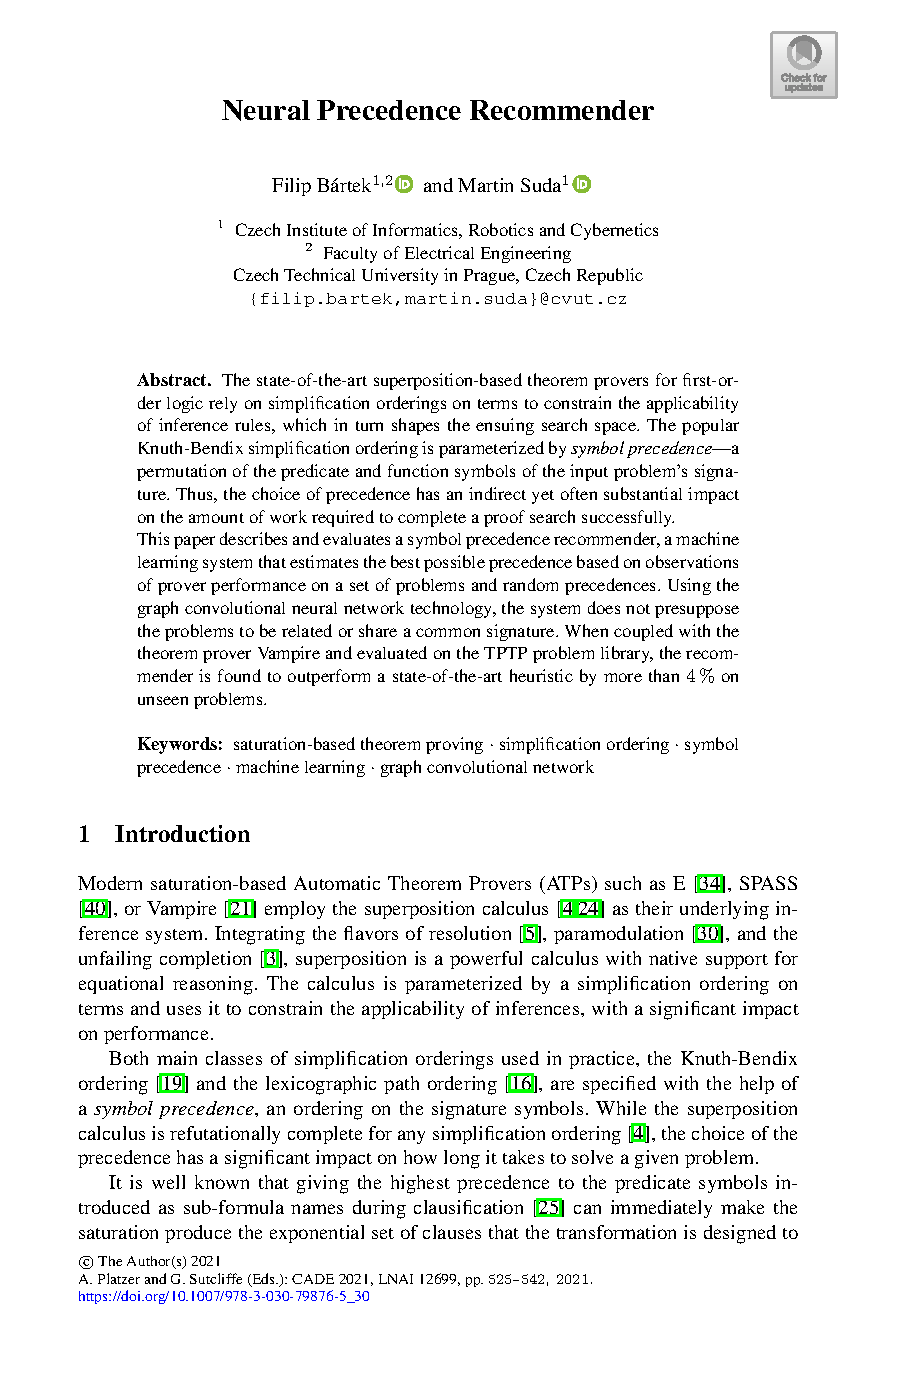
\includepdf[pages=-]{publications/Neural Precedence Recommender.pdf}

\section{A GNN-Advised Clause Selection}
\label{sec:results:gnn}

Filip Bártek and Martin Suda. How much should this symbol weigh? A \acrshort{gnn}-Advised Clause Selection \cite{DBLP:conf/lpar/Bartek023}

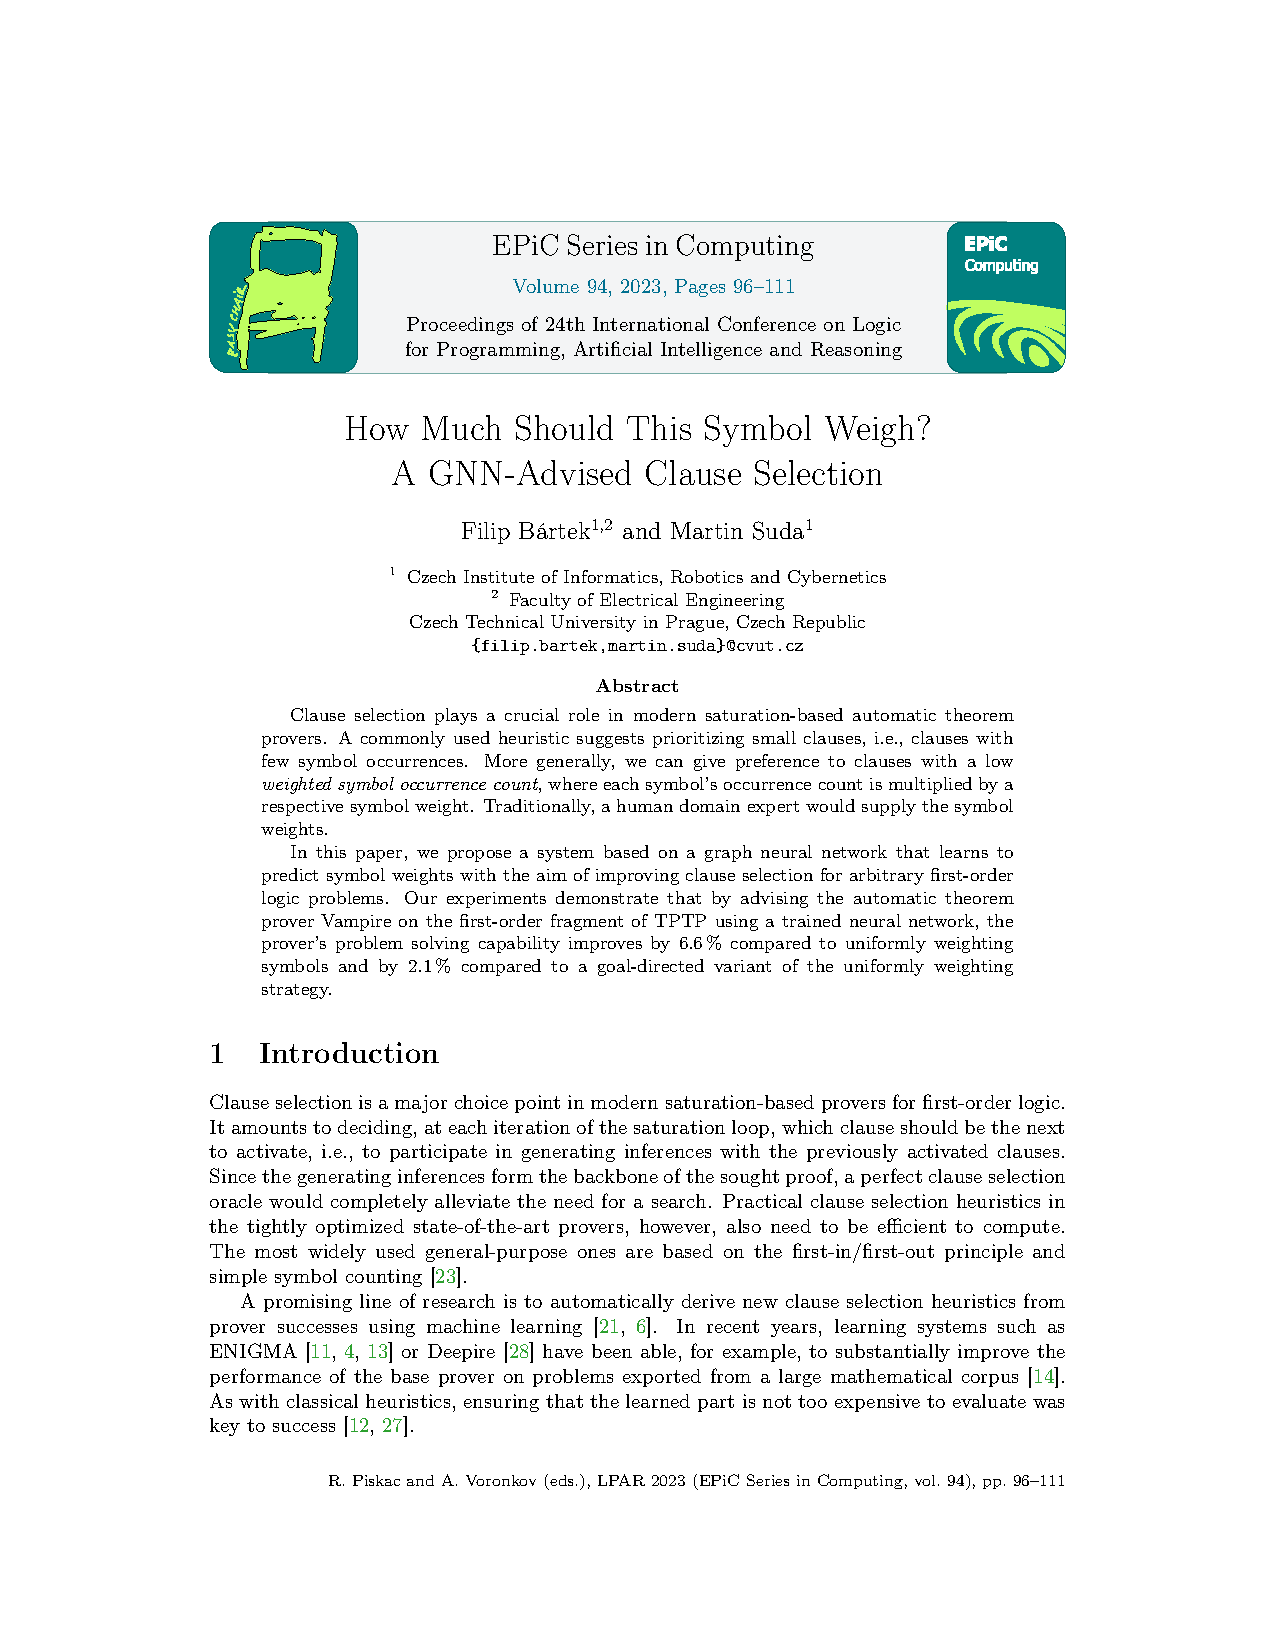
\includepdf[pages=-]{publications/weights.pdf}

\section{Regularization in Spider-Style Strategy Discovery and Schedule Construction}
\label{sec:results:regularization}

Filip Bártek, Karel Chvalovský, and Martin Suda. Regularization in Spider-Style Strategy Discovery and Schedule Construction. \Gls{ijcar}, 2024 (accepted). \cite{bartek2024regularization}\todo{Replace by the final version and link to the arXiv version with appendix.}

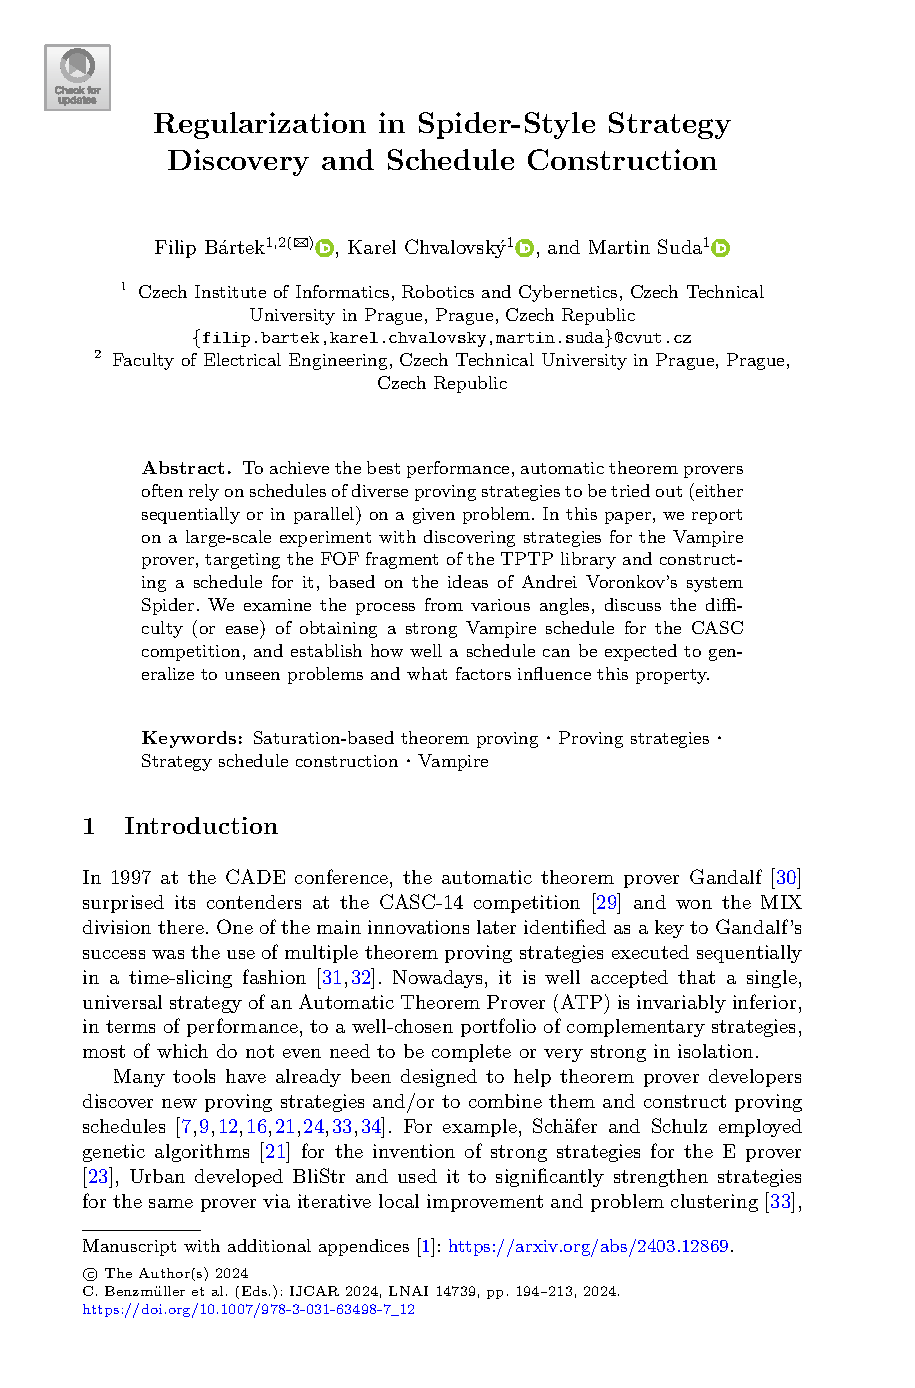
\includepdf[pages=-]{publications/regularization.pdf}

}

\chapter{Conclusion}

%e) v závěrečné části
%i) přehled výsledků disertace včetně původního přínosu doktoranda (tj.
%stručný přehled původních výsledků disertace, v čem zlepšují současný
%stav),
%ii) závěry pro další rozvoj vědy nebo pro realizaci v praxi,

\todo[inline]{TBA}

%\appendix
%\printindex

\appendix

\chapter{Author's Publications}

%f) a list of the candidate’s publications (projects) including their public acceptance
%(e.g. citations); the list shall be divided into publications related to the dissertation
%topics and other publications; in both sections, the publication shall be subdivided as
%follows: publications in impacted journals, peer reviewed journals, patents, further
%publications excerpted by WoS3 and others; (in case the share of all co-authors is not
%equal, the list shall be completed by the doctoral student’s share of co-authorship for
%individual publications; furthermore, these shares must be supported with a
%declaration of agreement by all the authors).

%f) seznam vlastních publikací (projektů) včetně jejich ohlasů; seznam je členěn
%na publikace vztahující se k tématu disertační práce a na publikace ostatní; v obou
%oddílech se publikace dělí následovně: publikace v impaktovaných časopisech,
%recenzovaných časopisech, patenty, další publikace excerpované WoS a
%publikace ostatní (ke každému článku je přiloženo prohlášení o příspěvku
%jednotlivých spoluautorů (Authorship Statement/Contribution), pokud toto
%prohlášení již není součástí článku dle ŘDS, čl. 7 odst. 3.

% Author contributions:
% https://credit.niso.org/
% https://credit.niso.org/contributor-roles-defined/
% https://www.springer.com/us/editorial-policies/authorship-principles#toc-49265

% Examples:
% https://www.elsevier.com/researcher/author/policies-and-guidelines/credit-author-statement
% https://link.springer.com/journal/11145/submission-guidelines#Instructions%20for%20Authors_Authorship%20principles
% https://onlinelibrary.wiley.com/doi/epdf/10.1087/20150211
% https://www.cell.com/pb/assets/raw/shared/guidelines/CRediT-taxonomy.pdf
% https://pubs.rsc.org/en/content/articlelanding/2023/DD/D2DD00099G

% My publications:
% https://docs.google.com/spreadsheets/d/1rHV33O5apSXxvtCM6_gqnm2dEmj-dV7ij-QQK0__85k

\newcommand{\auth}\emph
\newcommand{\core}[3]{\href{https://portal.core.edu.au/conf-ranks/#3/}{CORE#1 conference rank: #2}}
\newcommand{\wos}[1]{\href{https://www.webofscience.com/wos/woscc/full-record/WOS:#1}{Web of Science record: #1}}
%\newcommand{\citations}[3]{\href{https://scholar.google.com/citations?view_op=view_citation&citation_for_view=DiFzKOgAAAAJ:#3}{Number of citations according to Google Scholar: #1 (excluding self-citations: #2)}}
\newcommand{\scholar}{Source: \href{https://scholar.google.com/}{Google Scholar}. Date extracted: \DTMdisplaydate{2024}{9}{11}{-1}.}
\newcommand{\external}{Excluding self-citations.}
%\newcommand{\citations}[4]{\href{https://scholar.google.com/scholar?cites=#4}{Number of citations\footnote{\scholar{} \external{}}\todo{Join duplicate footnotes.}\todo{Unfiy the date format with the rest of the document.}: #2}}
\newcommand{\citations}[4]{\href{https://scholar.google.com/scholar?cites=#4}{Number of citations\footnote{\scholar{} \external{}}: #2}}

%\Cref{tab:publications} shows an overview of the publications.

%in case the share of all co-authors is not
%equal, the list shall be completed by the doctoral student’s share of co-authorship for
%individual publications

\todo[inline]{Consider removing the table.}
\begin{table}[h]
\begin{ctucolortab}
\centering
\caption{Conference and workshop publications. Each publication is identified by the event (conference or workshop) it was published at.}
\label{tab:publications}
\begin{tabular}{lr|ccrrcc}
%\toprule
\multirow{2}{*}{Event} & \multirow{2}{*}{Year} & \multirow{2}{*}{CORE\tablefootnote{CORE conference rank}} & \multirow{2}{*}{WoS\tablefootnote{Is the publication indexed in Web of Science?}} & \multicolumn{2}{c}{Citations\tablefootnote{\scholar}} & \multirow{2}{*}{Sect.} & \multirow{2}{*}{Bibliography} \\
& & & & All & Ext.\tablefootnote{\external} & & \\
\midrule
\Acrshort{paar}  & 2020 &   &   & 6 & 4 & \ref{sec:results:simple} & \cite{DBLP:conf/cade/Bartek020} \\
\Acrshort{cade}  & 2021 & A & \checkmark & 8 & 5 & \ref{sec:results:npr} & \cite{DBLP:conf/cade/Bartek021} \\
\Acrshort{lpar}  & 2023 & A &   & 3 & 1 & \ref{sec:results:selection} & \cite{DBLP:conf/lpar/Bartek023} \\
\Acrshort{ijcar} & 2024 & A & \checkmark & 3 & 1 & \ref{sec:results:regularization} & \cite{DBLP:conf/ijcar/BartekCS24} \\
\Acrshort{paar}  & 2024 &   &   &   &   & \ref{sec:results:cautious} & \cite{DBLP:conf/paar/BartekC024} \\
%\bottomrule
\end{tabular}
\end{ctucolortab}
\end{table}

\todo[inline]{Add detailed contributions.}
For each of the publications listed below,
the contributions of individual authors follow the \href{https://credit.niso.org/}{CRediT contributor role taxonomy} \cite{DBLP:journals/lp/BrandAAHS15}.
% Role descriptions: https://credit.niso.org/contributor-roles-defined/

\section{Publications Related to the Dissertation Thesis}
% publikace vztahující se k tématu disertační práce

\subsection{Publications Indexed in \href{https://www.webofscience.com/}{Web of Science}}
% další publikace excerpované WoS
\label{sec:wos}

\subsubsection{Neural Precedence Recommender}

\auth{Filip Bártek} and Martin Suda.
Neural Precedence Recommender.
\Acrfull{cade} 2021.
\cite{DBLP:conf/cade/Bartek021}
\\ \core{2021}{A}{918}
%\\ \wos{000693448800030}
\\ \citations{8}{5}{d1gkVwhDpl0C}{4757052500503566147}
\\ See \cref{sec:results:npr}.

\subsubsection{Regularization in Spider-Style Strategy Discovery and Schedule Construction}

%\auth{Filip Bártek}, Karel Chvalovský, and Martin Suda.
%Regularization in Spider-Style Strategy Discovery and Schedule Construction.
%\Acrfull{ijcar} 2024.
%\cite{DBLP:conf/ijcar/BartekCS24}

\begin{itemize}
\item[Authors] \auth{Filip Bártek}, Karel Chvalovský, and Martin Suda
\item[Title] Regularization in Spider-Style Strategy Discovery and Schedule Construction \cite{DBLP:conf/ijcar/BartekCS24}
\item[Conference] \Acrfull{ijcar} 2024\footnote{\core{2023}{A}{1314}}
%\item \wos{001273489700012}
%\item \citations{3}{1}{IjCSPb-OGe4C}{14661423119916603256}
\item[Public acceptance] \citations{3}{1}{IjCSPb-OGe4C}{14661423119916603256}
\end{itemize}

This paper is included in \cref{sec:results:regularization}.

\paragraph{Author contributions.}
Conceptualization: M.S., \auth{F.B.}, and K.C.;
Data curation: \auth{F.B.} and M.S.;
Formal analysis: \auth{F.B.} and M.S.;
Funding acquisition: M.S., \auth{F.B.}, and Josef Urban;
Investigation: \auth{F.B.}, M.S., and K.C.;
Methodology: M.S., \auth{F.B.}, and K.C.;
Project administration: M.S.;
Resources: Josef Urban;
Software: \auth{F.B.}, M.S., and K.C.;
Supervision: M.S.;
Validation: \auth{F.B.};
Visualization: \auth{F.B.} and M.S.;
Writing -- original draft: M.S., \auth{F.B.}, and K.C.;
Writing -- review \& editing: \auth{F.B.}, M.S., and K.C.

\subsection{Other Publications}
% publikace ostatní

\subsubsection{Conference and Workshop Papers}

\begin{enumerate}

\item \auth{Filip Bártek} and Martin Suda.
Learning Precedences from Simple Symbol Features.
\Acrfull{paar} 2020.
\cite{DBLP:conf/cade/Bartek020}
\\ \citations{6}{4}{u-x6o8ySG0sC}{7330041666500653943}
\\ See \cref{sec:results:simple}.

\item \auth{Filip Bártek} and Martin Suda.
How much should this symbol weigh? A \acrshort{gnn}-Advised Clause Selection.
\Acrfull{lpar} 2023.
\cite{DBLP:conf/lpar/Bartek023}
\\ \core{2021}{A}{1596}
\\ \citations{3}{1}{qjMakFHDy7sC}{3677938196667465426}
\\ See \cref{sec:results:selection}.

\item \auth{Filip Bártek}, Karel Chvalovský, and Martin Suda.
Cautious Specialization of Strategy Schedules (Extended Abstract).
\Acrfull{paar} 2024.
\cite{DBLP:conf/paar/BartekC024}
\\ See \cref{sec:results:cautious}.

\end{enumerate}

%\subsubsection{Extended abstracts}

\subsubsection{Datasets}

\begin{enumerate}
\item \auth{Filip Bártek} and Martin Suda.
Vampire strategy performance measurements.
2024.
\cite{bartek10814478}
\end{enumerate}

%\section{Unrelated Publications}
%% publikace ostatní
%\todo[inline]{Should I only include publications created during the PhD? If yes, remove this section.}
%
%\begin{enumerate}
%\item \auth{Filip Bártek}. \foreignlanguage{czech}{Realizace Rabinovy hry na konečných grafech}. Bachelor's thesis. 2012. \cite{Bartek2012thesis}
%\item \auth{Filip Bártek}. Minimum representations of Boolean functions defined by multiple intervals. Master's thesis. 2015. \cite{bartek2015}
%\end{enumerate}


\printglossaries

\bibliography{bartefil}

\ctutemplate{specification.as.chapter}

\end{document}
